\documentclass[tikz,border=2mm]{standalone}
\tikzset{global scale/.style={
    	scale=#1,
    	every node/.append style={scale=#1}
  	}
}
\begin{document}
	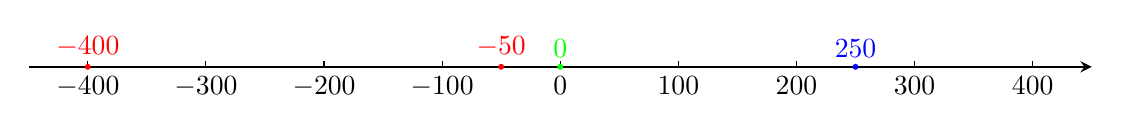
\begin{tikzpicture}[scale = 0.015]
  		\draw [black, thick, ->, >=stealth] (-450,0) -- (450,0);
		\foreach \x in {-400,-300,...,400}
			\draw (\x,5) -- (\x,0) node[anchor=north] {$\x$};
		% (2) - 50, 250, 0, -400
		\draw [red, fill=red] (-50, 0) circle(2) node [above] {$-50$}; 
		\draw [red, fill=red] (-400, 0) circle(2) node [above] {$-400$}; 	
		\draw [green, fill=green] (0, 0) circle(2) node [above] {$0$}; 		
		\draw [blue, fill=blue] (250, 0) circle(2) node [above] {$250$}; 
	\end{tikzpicture}    
\end{document}
